\section{Preguntas largas}
% Ordenadas por orden de aparición en los temas
\subsection{Enumera y comenta las principales características del software asociadas a su naturaleza ``inmaterial''}
\textit{Tema 1 Apartado 1}

\subsection{Enumera y comenta los principales problemas crónicos del software}
\textit{Tema 1 Apartado 4}

\subsection{Norma 12207-1: Procesos de soporte. ¿Cuál es su diferencia fundamental con la 1074? ¿Qué aporta la 15504-2 que no contempla la 12207 en los procesos de la organización?}
\textit{Tema 2 Apartado 2.1, 2.2, 2.3}

% \subsection{¿En qué consiste el modelo de capacidad CMMI?, diferencias con respecto al modelo de madurez.}
% %\textit{Tema 2 Apartado 3.1}
% Esta pregunta \textbf{NO} se refiere a la diferencia entre CMMI continuo y discreto sino a la diferencia entre CMM y CMMI, debido a que \textbf{CMM no aparece actualmente en las transparencias} del Rabenso asumimos que no existe.

\subsection{Describe en qué consiste el ciclo de vida en espiral, cuales son sus ventajas e inconvenientes. Describe la metodología para el análisis de riesgos según Sommerville}
\textit{Tema 2 Apartado 5}


\subsection{Para cada uno de los siguientes diagramas, señala los elementos que contienen y describe su función en el diagrama}

\begin{figure}[H]
  \centering
  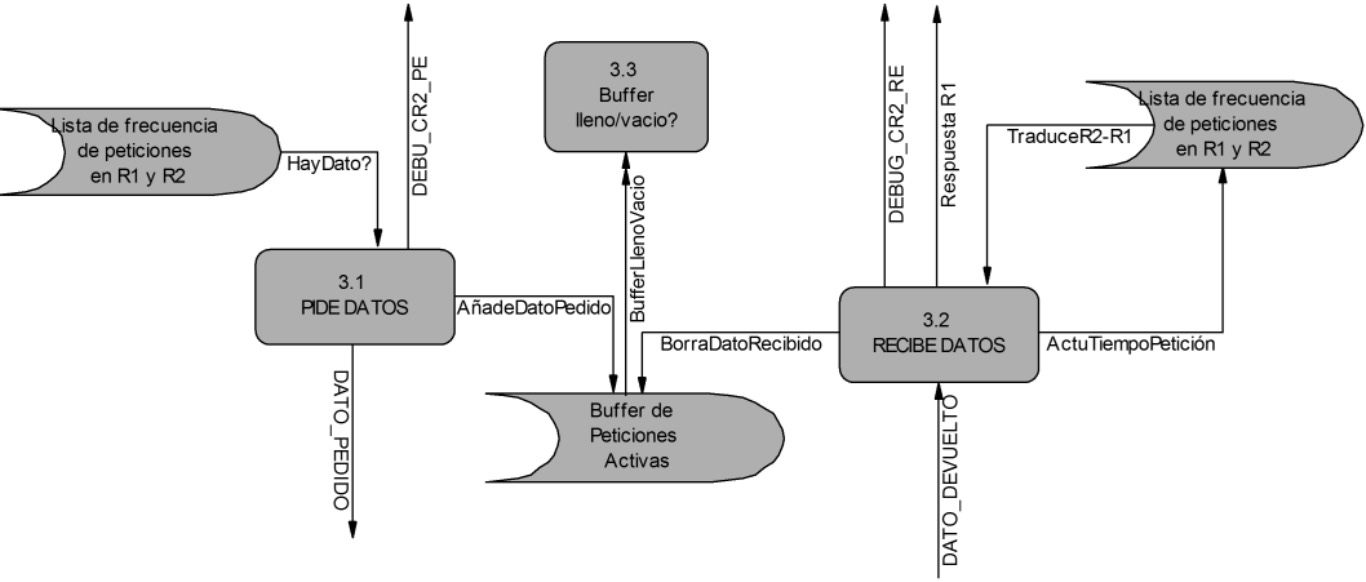
\includegraphics[width=0.8\linewidth]{Resources/diagramaA}
\end{figure}

\begin{figure}[H]
  \centering
  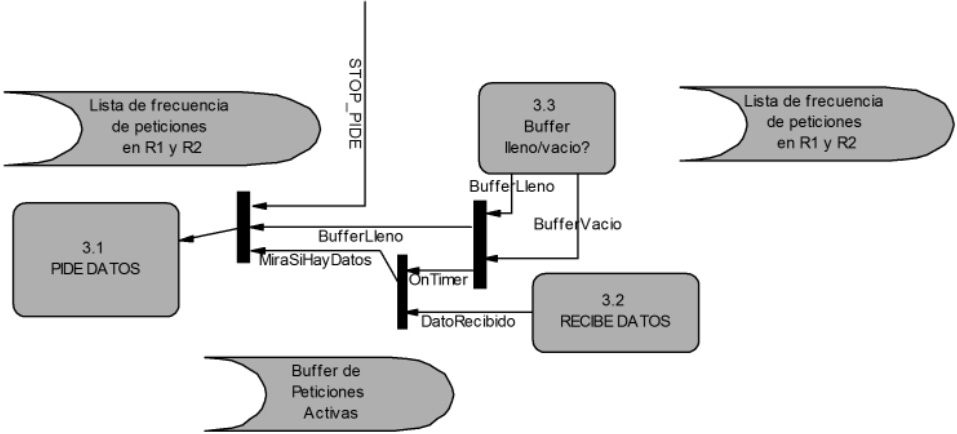
\includegraphics[width=0.8\linewidth]{Resources/diagramaB}
\end{figure}

\textit{Tema 5 Apartado 2.3}




\subsection{Comenta el proceso de elaboración de un plan de prueba seguido por el estándar IEEE 829 y los documentos asociados al proceso ¿Cuál es el estándar de ejecución de las pruebas? ¿Qué documentación implica?}
\textit{Tema 6 Apartado 3}

\subsubsection{Describe en qué consisten las pruebas funcionales, para qué sirven, en base a qué se construyen. Describe en detalle 3 técnicas de construcción de este tipo de pruebas.}
\textit{Tema 6 Apartado 4.1}

